\section{Introduction}
\label{introduction}
VTK is an open source cross-platform software system used for scientific data
processing, analysis, and visualization. It was originally developed to supplement a textbook on object oriented computer graphics
programming~\citep{schroeder_visualization_2006, geveci_vtk_2012}.  Since its
inception, VTK has a long history of volume rendering and, unfortunately, that
history was evident in the large collection of classes used to render
volumes. While these methods were state-of-the-art at the time they were
implemented, given VTK's 20+ year history, many of these methods are now
obsolete. Recently, there has been a major
effort~\citep{hanwell_visualization_2015} undertaken to re-write VTK's rendering
backend originally based on a legacy, now-deprecated OpenGL API to one based on a modern programmable
pipeline OpenGL API~\citep{shreiner_opengl_2013}. This new rendering subsystem was designed to support the latest
technological advances in the graphics hardware industry. Consequently one of the objectives of
the work was to consolidate the number of volume mappers to two: one
supporting accelerated rendering using the Graphics Processing Unit (GPU) and
a second, parallel implementation on the Central Processing Unit (CPU). In addition, a
\texttt{vtkSmartVolumeMapper} class was added to assist application developers provide automatic
run-time selection of the appropriate volume rendering techniques based on system configuration.

\begin{figure}[ht]
  \centering
  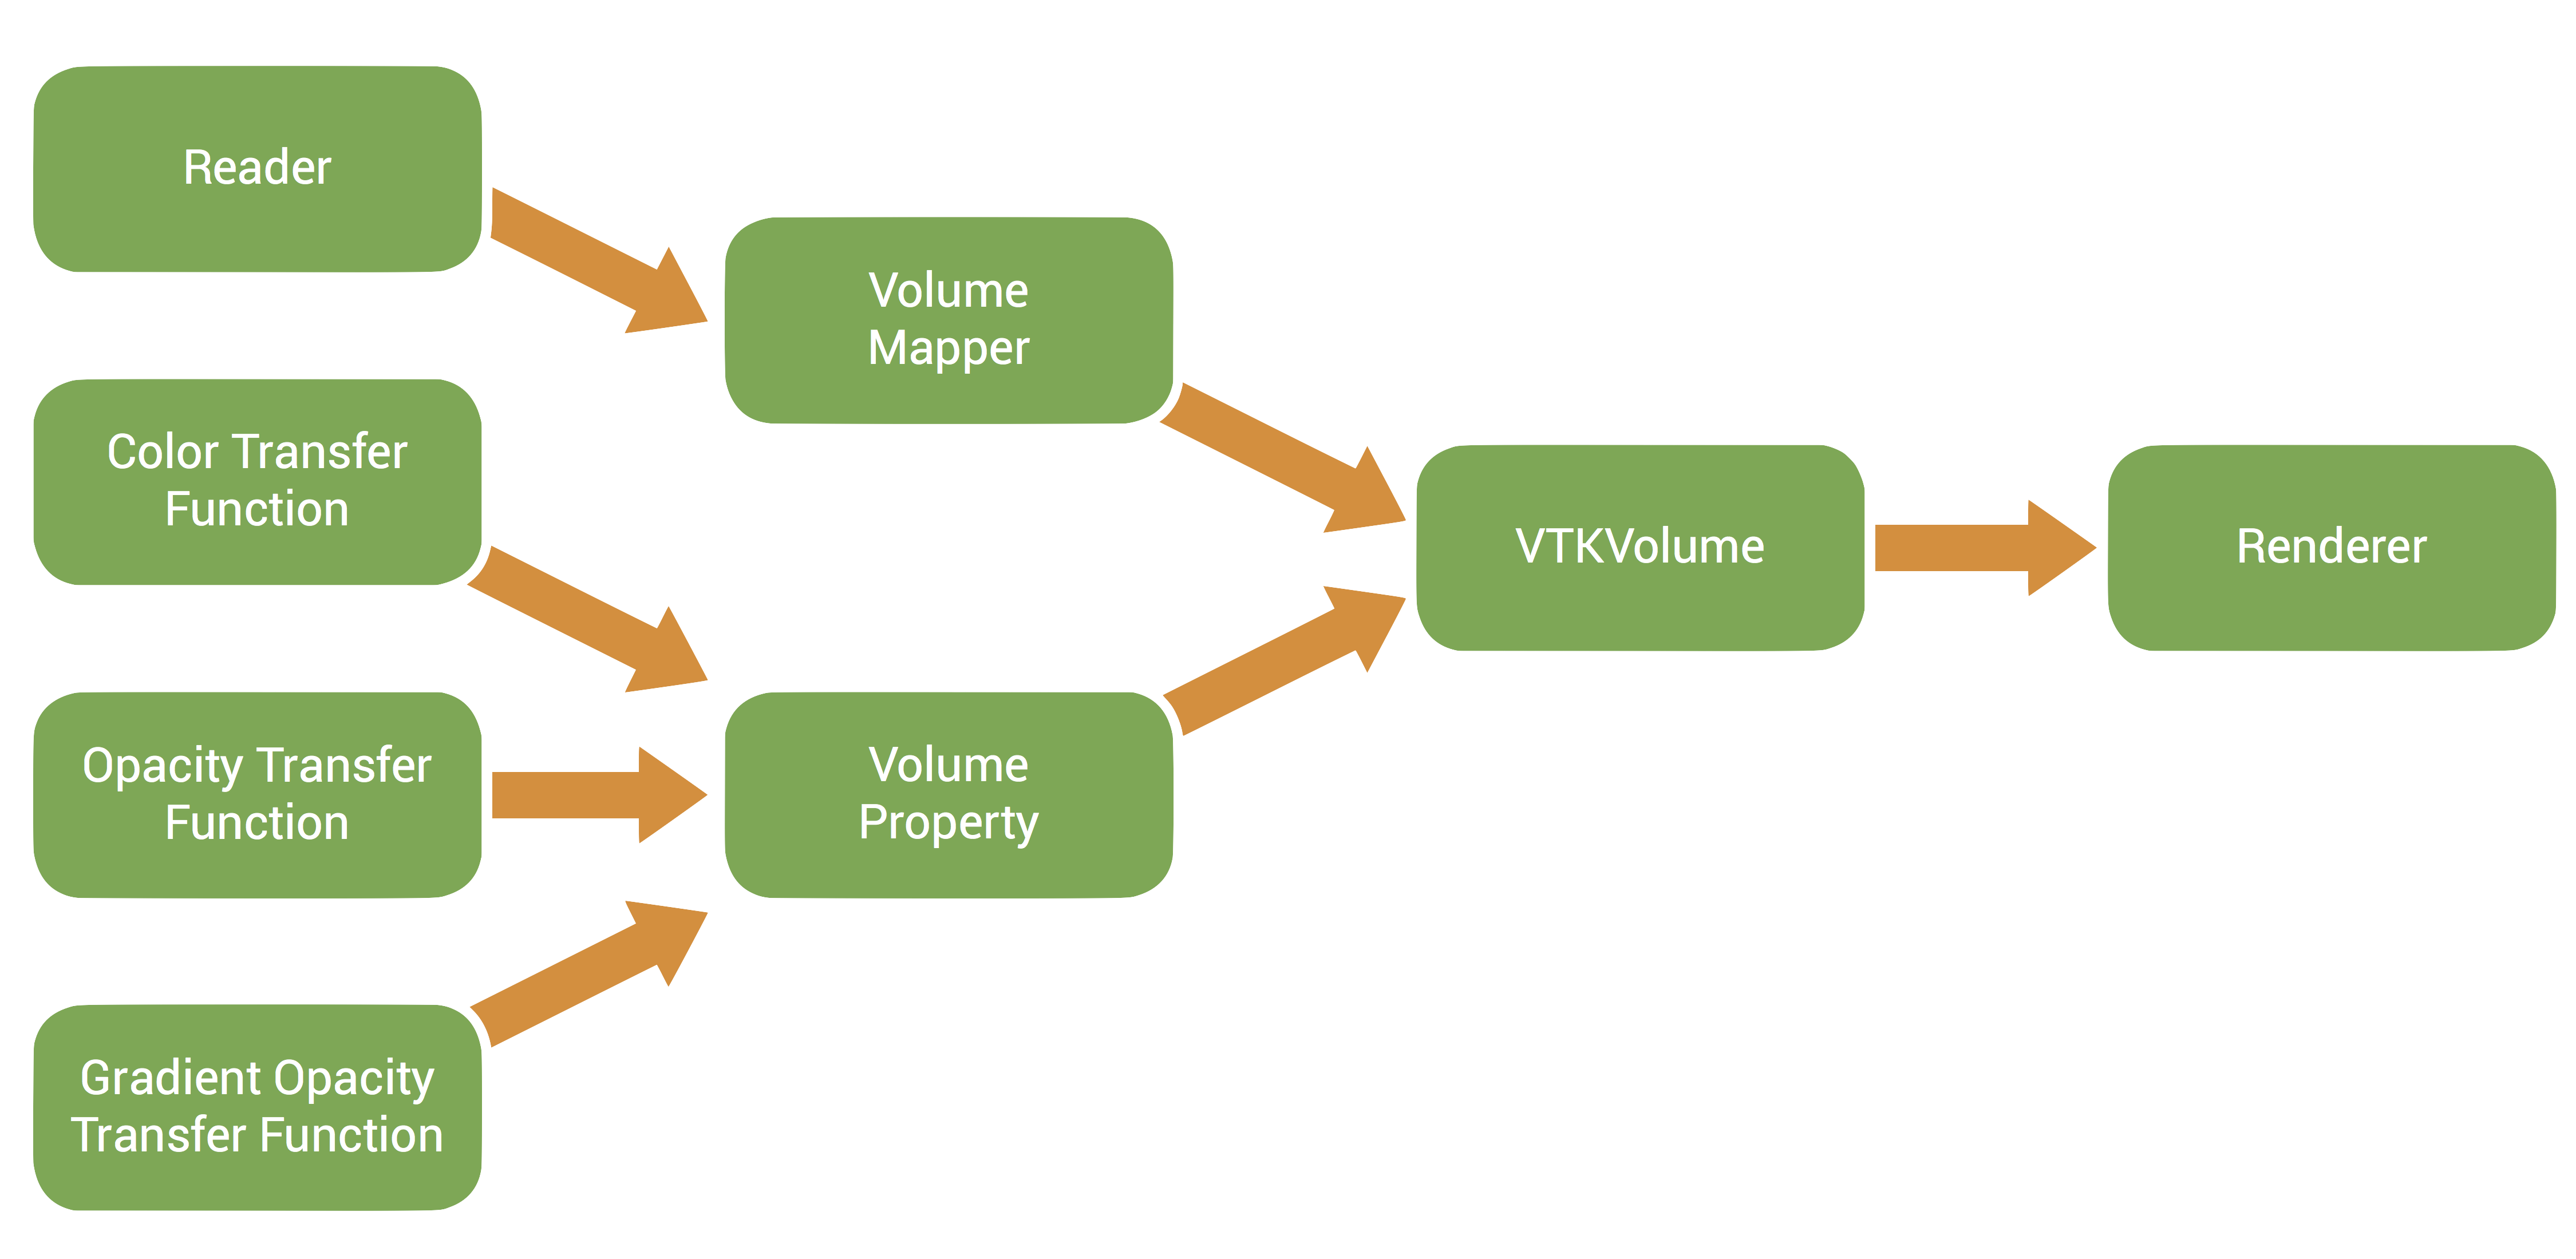
\includegraphics[width=\columnwidth]{vtk_volume_pipeline.png}
  \caption{VTK pipeline for volume rendering which is similar to VTK polygonal
    rendering with differences such as transfer functions are defined on the
    property object.}
  \label{fig:pipeline}
\end{figure}%

Thus a primary objective of this OpenGL modernization effort, and the
subject of this article, was to create a cross-platform, multi-functional,
high-performance volume renderer supporting both serial and parallel execution
modes capable of supporting such complex applications as
ParaView~\citep{ahrens_paraview:_2005,ayachit_paraview_2015} or 3D
Slicer~\citep{fedorov_3d_2012}.
In addition our effort addressed the following key requirements:

\begin{itemize}
  \item Enable ubiquitous, cross-platform, high-performance support for volume
    rendering across all major operating systems and computing environments (desktop, VR, mobile).

  \item Ensure that the new volume visualization subsystem provides support for VTK-based pipeline and data-flow
    networks, thereby providing a flexible system addressing a wide variety of scientific and medical data
    visualization use-cases.

  \item Provide a variety of useful features at interactive frame
    rates such as clipping, cropping, gradient opacity, mixed geometry-volume translucent
    rendering, and on-demand shader composition.
\end{itemize}

To achieve this, we created a replacement for the OpenGL fixed pipeline based
vtkGPUVolumeRayCastMapper. The new mapper, which shares the same name but uses
a modern OpenGL programmable pipeline, can be used via
\texttt{vtkSmartVolumeMapper} or instantiated directly. Availability of the
new mapper with the new OpenGL-VTK implementation improves the management of
textures in the mapper and benefits both forms of rendering (geometry and
volume) by sharing common code between them. While volume ray-casting itself
is a well-known technique, developing a volume renderer that works with
variety of data formats and types, supports many essential features for
medical and scientific computing, works across all major computing platforms,
and performs well at interactive frame rates with very large datasets was a
challenging task that required an in-depth knowledge of the data, graphics
pipeline, VTK framework, and user requirements.  In the next section, we
describe the technical details behind the effort to produce the resulting
modern, cross-platform volume renderer delivered to the open source VTK
community.
